
\documentclass[11pt]{article}
\usepackage[a4paper,margin=1in]{geometry}
\usepackage[T1]{fontenc}
\usepackage[utf8]{inputenc}
\usepackage{lmodern,microtype}
\usepackage{amsmath,amssymb,amsthm,mathtools}
\usepackage{graphicx,booktabs,float,enumitem}
\usepackage{xcolor}
\usepackage[colorlinks=true,linkcolor=blue!55!black,citecolor=blue!55!black,urlcolor=blue!55!black]{hyperref}
\usepackage[nameinlink,capitalise,noabbrev]{cleveref}

\newtheorem{theorem}{Theorem}[section]
\newtheorem{proposition}[theorem]{Proposition}
\newtheorem{corollary}[theorem]{Corollary}
\theoremstyle{definition}
\newtheorem{definition}[theorem]{Definition}
\newtheorem{remark}[theorem]{Remark}
\newtheorem{example}[theorem]{Example}
\newcommand{\C}{\mathbb C}
\newcommand{\widehatC}{\widehat{\mathbb C}}

\title{Complex Dynamics of Equal-Value Pole Maps\\
\large Anchored Divided Differences, Pole Geometry, and Anchor Bifurcations}
\author{Ivan Besevic\\Independent Mathematical Research\\\texttt{github.com/ivan-fr/poussiere\_de\_x}}
\date{May 2026}

\begin{document}
\maketitle

\begin{abstract}
For an analytic equation $F(z)=0$, the anchored divided-difference map
\[
P_{F,a}(z)=a-\frac{F(a)}{F[a,z]}
=a-\frac{F(a)(a-z)}{F(a)-F(z)}
\]
has roots of $F$ as fixed points and has poles at the equal-value set $F(z)=F(a)$. In the complex plane this produces a meromorphic dynamical system whose pole geometry is fundamentally different from Newton dynamics. Newton poles are controlled by critical points of $F$; anchored Pandrosion poles are controlled by level sets of $F$. This paper develops the basic complex dynamics of these equal-value pole maps. For polynomial $F$, $P_{F,a}$ is a rational map whose fixed points are exactly the roots of $F$ away from the anchor, whose poles are the non-anchor points in $F^{-1}(F(a))$, and whose critical points solve
\[
F(a)-F(z)-(a-z)F'(z)=0.
\]
The local multiplier at a root is
\[
\lambda_r(a)=1-\frac{(a-r)F'(r)}{F(a)}.
\]
Thus anchor motion changes both the local attraction at roots and the global pole skeleton. Figures for $F(z)=z^3-1$ show basin changes, equal-value pole motion, and anchor-parameter regions where all root multipliers are small. The result is a proposed new dynamical viewpoint: anchored maps encode the level-set geometry of $F$ directly into their poles.
\end{abstract}

\paragraph{One-sentence summary.}
Anchored divided-difference dynamics replaces Newton's critical-point pole geometry by equal-value pole geometry: the poles are $F^{-1}(F(a))$.

\section{Introduction}

The scalar anchored Pandrosion map
\[
P_{F,a}(z)=a-\frac{F(a)}{F[a,z]}
\]
is a fixed-anchor secant map. On the real line its main role is local residual control. Over the complex plane it becomes a meromorphic map, and the location of its poles becomes a central dynamical object.

The essential difference from Newton's method is immediate. Newton's map is
\[
N_F(z)=z-\frac{F(z)}{F'(z)},
\]
so its poles occur where $F'(z)=0$. The anchored map is instead
\[
P_{F,a}(z)=a-\frac{F(a)(a-z)}{F(a)-F(z)},
\]
so its poles occur where
\[
F(z)=F(a).
\]
Thus the anchor does not merely set a local contraction factor; it selects a level set of $F$ and inserts that level set into the global rational dynamics.

\paragraph{Main questions.}
This paper organizes the first layer of this dynamics:
\begin{enumerate}[label=(\roman*)]
\item Which fixed points and poles does $P_{F,a}$ have?
\item How does the root multiplier change with the anchor?
\item What are the critical points of the rational map?
\item How do basins change as the anchor moves?
\end{enumerate}

\section{The equal-value pole map}

Let $F$ be a nonconstant polynomial or meromorphic function and choose an anchor $a$ with $F(a)\neq0$.

\begin{definition}[Equal-value pole map]
The anchored equal-value pole map is
\begin{equation}\label{eq:P}
P_{F,a}(z)=a-\frac{F(a)(a-z)}{F(a)-F(z)}.
\end{equation}
When $z=a$ is a removable point and $F'(a)\neq0$, one inserts the value
\[
P_{F,a}(a)=a-\frac{F(a)}{F'(a)}.
\]
\end{definition}

\begin{proposition}[Fixed points and poles]\label{prop:fixedpoles}
Assume $F(a)\neq0$.
\begin{enumerate}[label=(\alph*)]
\item If $F(r)=0$ and $r\neq a$, then $P_{F,a}(r)=r$.
\item If $P_{F,a}(z)=z$ and $z\neq a$ is not a pole, then $F(z)=0$.
\item The non-removable poles are contained in
\[
\Pi_{F,a}=\{z\neq a:F(z)=F(a)\}.
\]
\end{enumerate}
\end{proposition}

\begin{proof}
The fixed-point proof is the scalar divided-difference proof. If $F(r)=0$, then $F[a,r]=F(a)/(a-r)$, so $P_{F,a}(r)=r$. Conversely, $P_{F,a}(z)=z$ gives $F(a)-F(z)=F(a)$, hence $F(z)=0$. The pole statement follows directly from the denominator in \eqref{eq:P}.
\end{proof}

\begin{remark}
For $F(z)=z^p-x$ and anchor $a=1$, the equal-value poles satisfy $z^p=1$. The non-anchor poles are therefore the nontrivial roots of unity, recovering the cyclotomic pole geometry of the monomial theory.
\end{remark}

\section{Rational form, multipliers, and critical points}

If $F$ is a polynomial, then
\begin{equation}\label{eq:ratform}
P_{F,a}(z)=\frac{F(a)z-aF(z)}{F(a)-F(z)}.
\end{equation}
This is a rational map on $\widehat C$ after removable factors are cancelled.

\begin{proposition}[Root multiplier]\label{prop:mult}
If $r$ is a simple root of $F$ and $a\neq r$, then
\[
P'_{F,a}(r)=1-\frac{(a-r)F'(r)}{F(a)}.
\]
\end{proposition}

\begin{proof}
Differentiate \eqref{eq:P} or use the exact anchored multiplier identity.
\end{proof}

\begin{proposition}[Critical equation]\label{prop:critical}
Away from poles and removable points, the critical points of $P_{F,a}$ satisfy
\begin{equation}\label{eq:crit}
F(a)-F(z)-(a-z)F'(z)=0.
\end{equation}
\end{proposition}

\begin{proof}
Let $H(z)=F(a)-F(z)$. From \eqref{eq:P},
\[
P'_{F,a}(z)=F(a)\frac{H(z)-(a-z)F'(z)}{H(z)^2}.
\]
Thus critical points satisfy \eqref{eq:crit}.
\end{proof}

\begin{remark}
Equation \eqref{eq:crit} says that the critical points are those where the secant slope from the anchor equals the tangent slope at $z$:
\[
\frac{F(a)-F(z)}{a-z}=F'(z).
\]
Thus criticality is also a geometric secant-tangent condition.
\end{remark}

\section{Anchor bifurcation}

The anchor parameter $a$ affects the dynamics in two coupled ways:
\begin{enumerate}[label=(\arabic*)]
\item it changes the root multipliers $\lambda_r(a)$;
\item it moves the equal-value pole set $\Pi_{F,a}$.
\end{enumerate}
This is unlike Newton dynamics, where the pole set is tied to $F'$ and does not move with an external anchor.

\begin{definition}[Multiplier profile]
For a polynomial with simple roots $r_1,\dots,r_d$, define
\[
\Lambda(a)=\max_{1\le j\le d}\left|1-\frac{(a-r_j)F'(r_j)}{F(a)}\right|.
\]
A root-uniformly attracting anchor is one with $\Lambda(a)<1$.
\end{definition}

This definition is local. It does not guarantee global convergence, because global basins can be interrupted by equal-value poles. It does identify anchor regions where all roots are locally attracting.

\section{Example: \texorpdfstring{$F(z)=z^3-1$}{F(z)=z^3-1}}

Let $F(z)=z^3-1$. The roots are $1,\zeta,\zeta^2$, where $\zeta=e^{2\pi i/3}$. For an anchor $a$ with $a^3\neq1$, the non-removable equal-value poles solve
\[
z^3=a^3,\qquad z\neq a,
\]
so they are
\[
\zeta a,\qquad \zeta^2 a.
\]
Thus pole motion is completely visible: moving the anchor rotates two pole companions around it.

\begin{figure}[H]
\centering
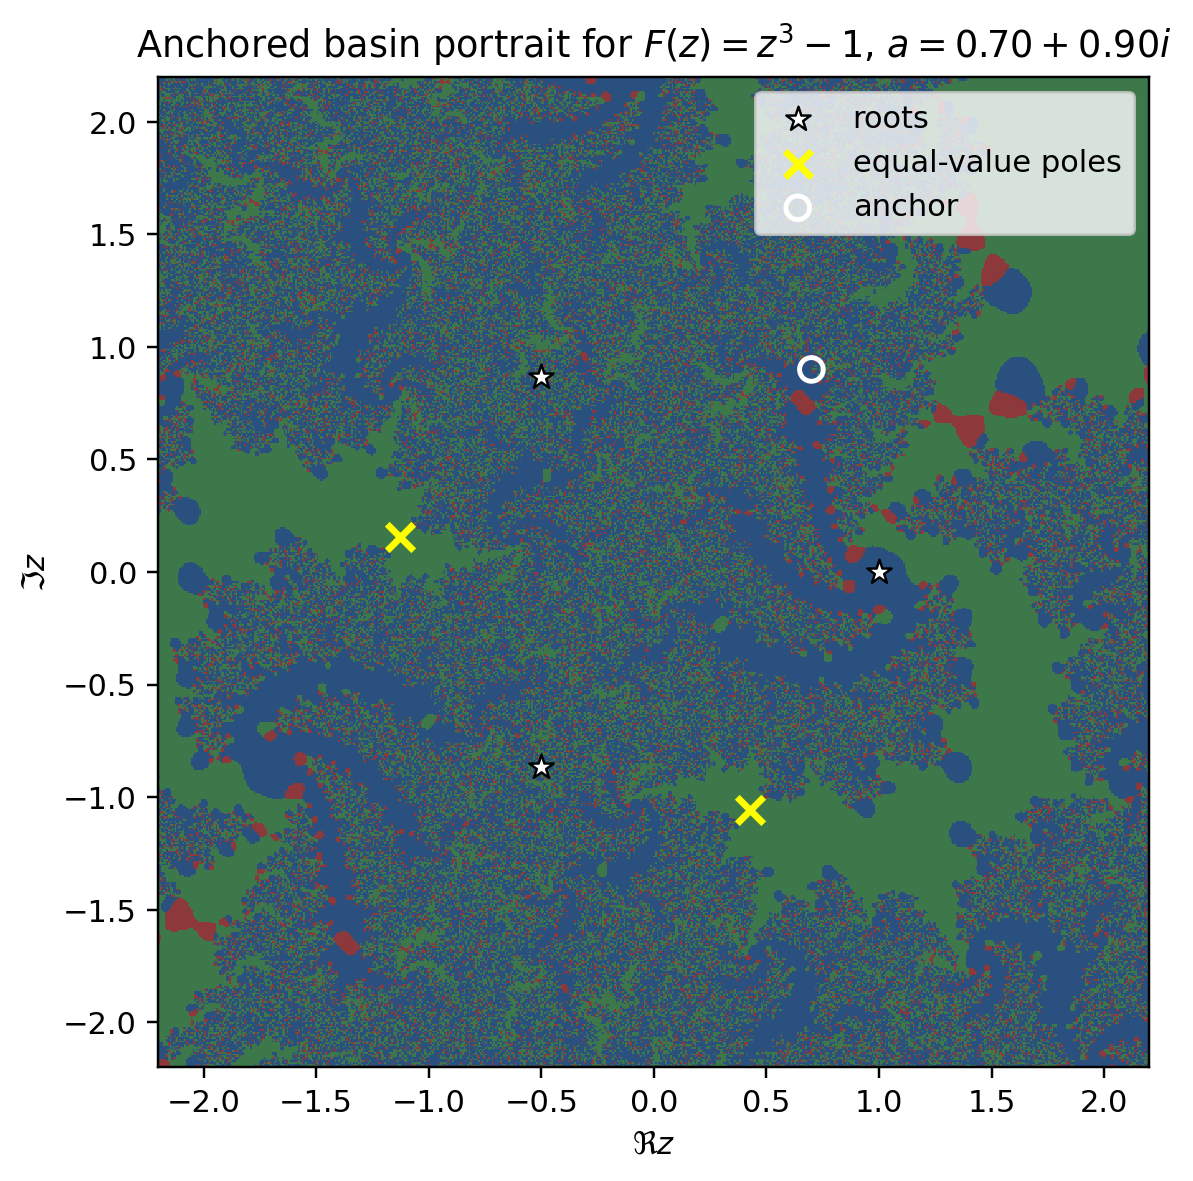
\includegraphics[width=.73\textwidth]{../figures/fig_basin_anchor_1.png}
\caption{Basins for $F(z)=z^3-1$ with anchor $a=0.70+0.90i$. The star markers are roots; yellow crosses mark the equal-value poles $\zeta a$ and $\zeta^2a$.}
\end{figure}

\begin{figure}[H]
\centering
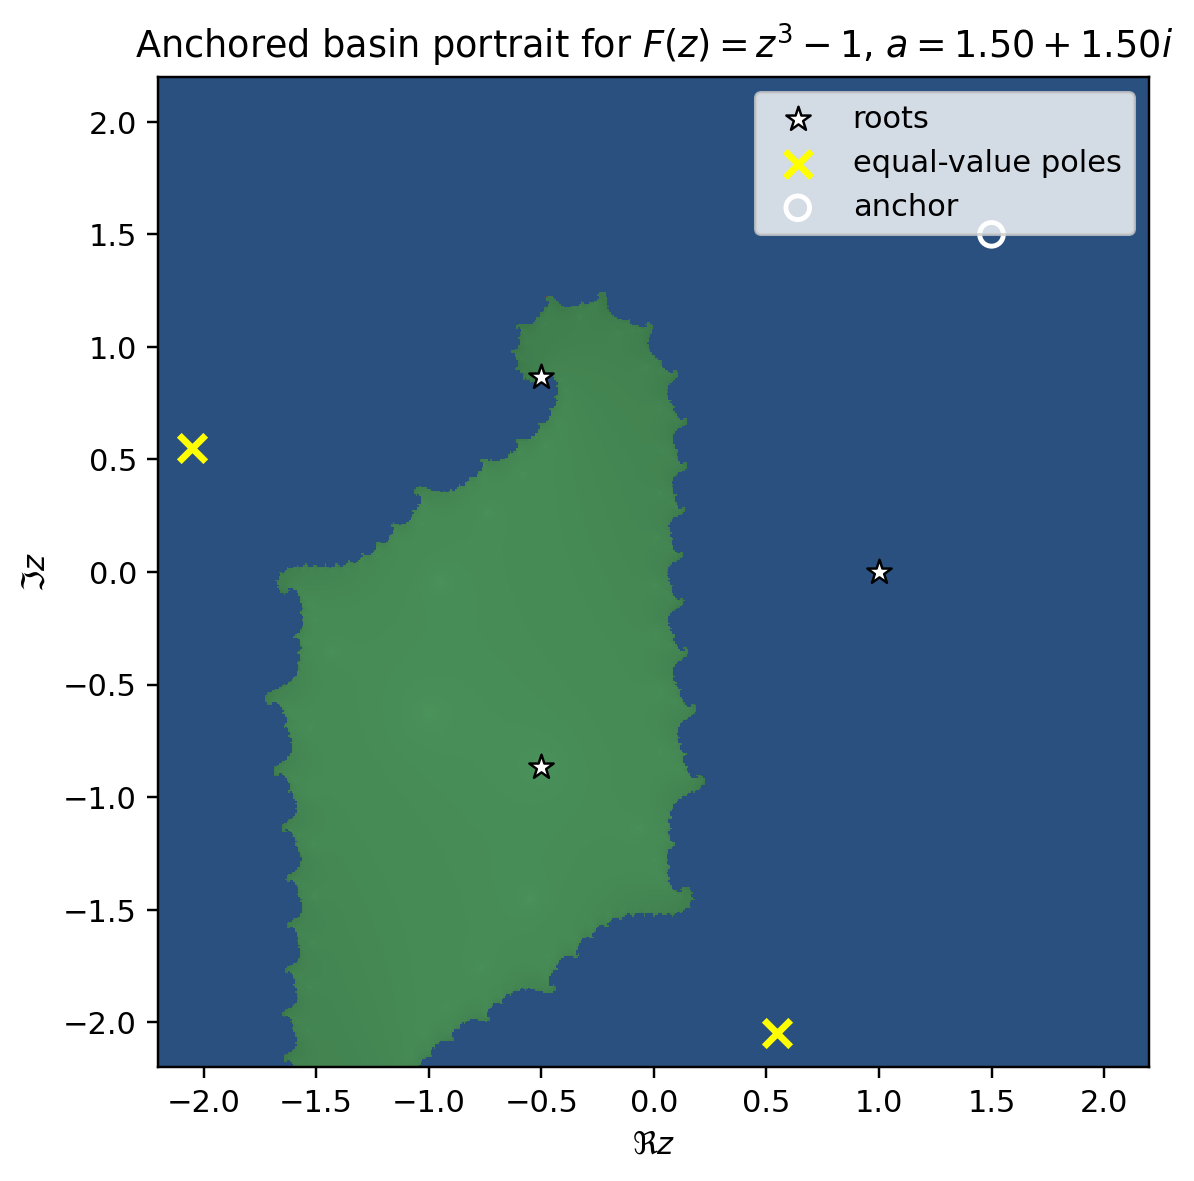
\includegraphics[width=.73\textwidth]{../figures/fig_basin_anchor_2.png}
\caption{Changing the anchor changes both the pole skeleton and the basin geometry. The poles are not fixed critical points of $F$; they are points on the anchor level set $F^{-1}(F(a))$.}
\end{figure}

\begin{figure}[H]
\centering
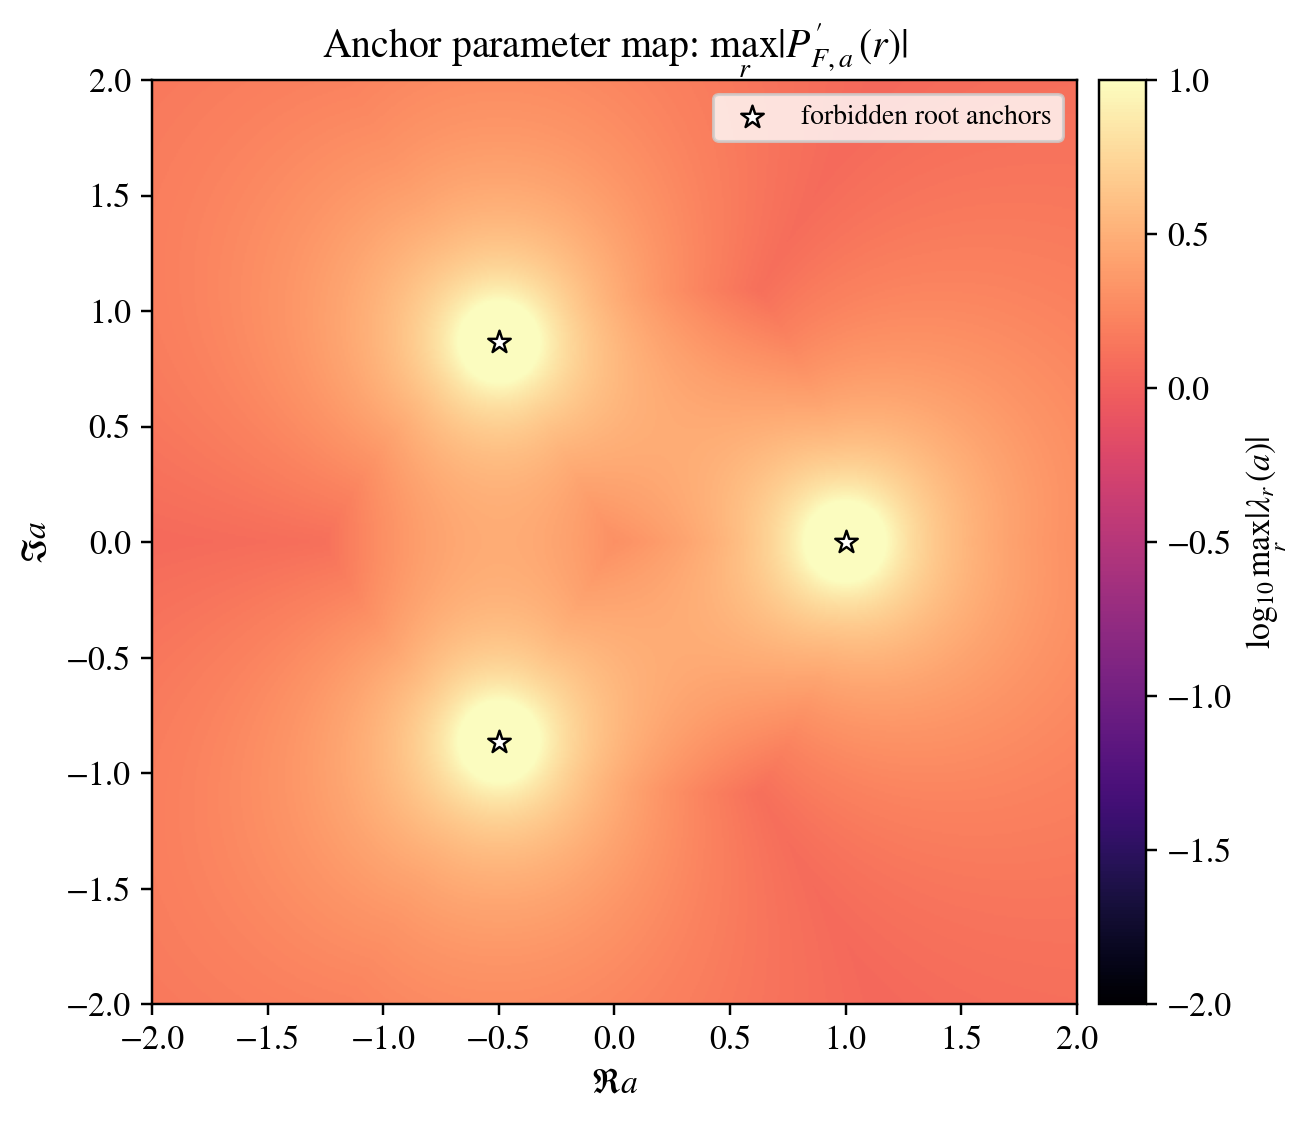
\includegraphics[width=.77\textwidth]{../figures/fig_anchor_parameter_multiplier.png}
\caption{Anchor-parameter map for $\Lambda(a)=\max_r|\lambda_r(a)|$. Darker regions have smaller worst root multiplier. The roots are excluded anchor values because $F(a)=0$.}
\end{figure}

\begin{figure}[H]
\centering
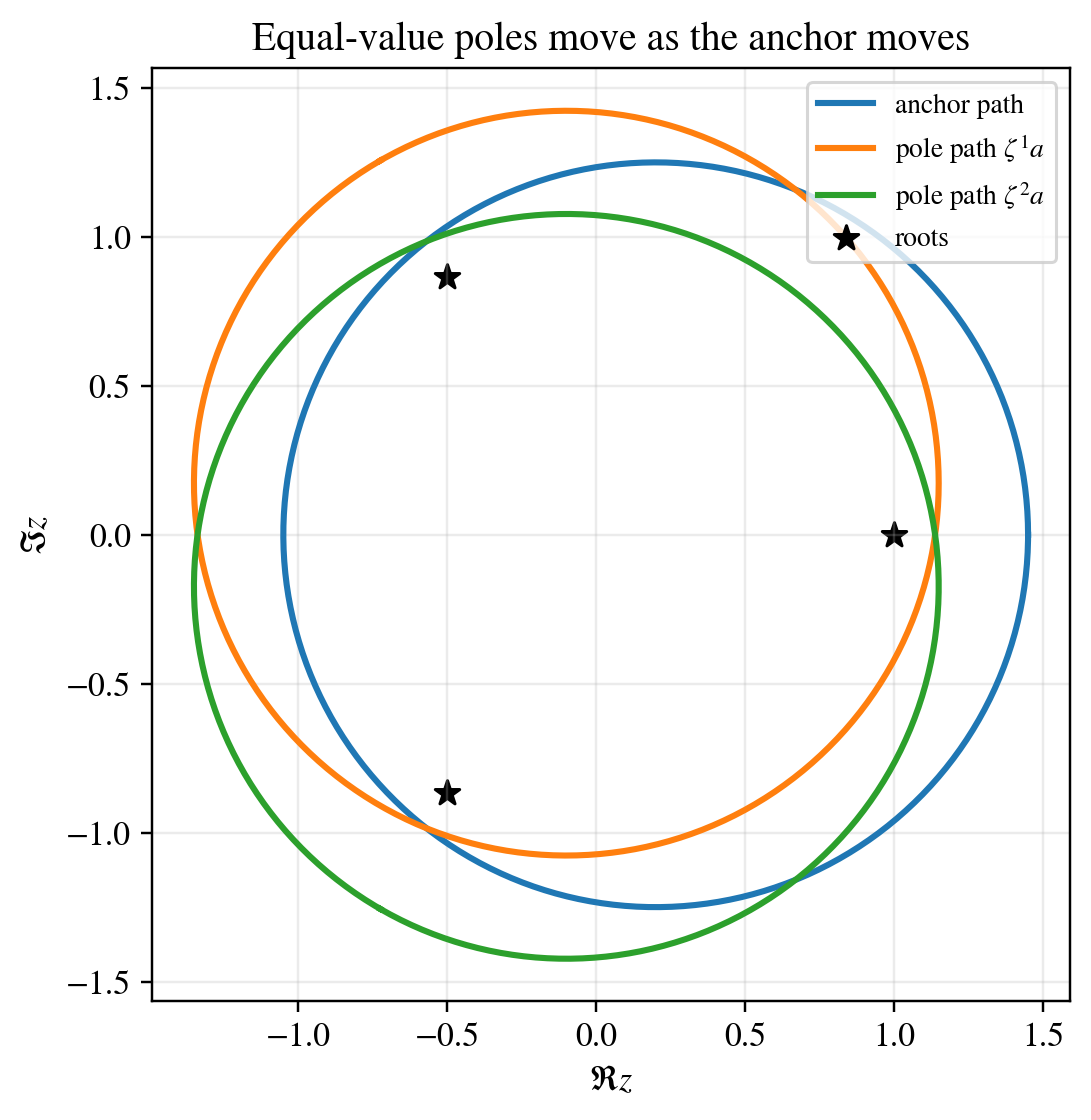
\includegraphics[width=.75\textwidth]{../figures/fig_equal_value_pole_motion.png}
\caption{Equal-value pole motion for $F(z)=z^3-1$. Along an anchor path, the two pole companions are $\zeta a$ and $\zeta^2a$. This is the simplest visible form of equal-value pole geometry.}
\end{figure}

\section{Comparison with Newton dynamics}

Newton's method and anchored divided-difference dynamics share roots as fixed points, but their global skeletons are different:
\[
N_F(z)=z-\frac{F(z)}{F'(z)}
\quad\Rightarrow\quad
\text{poles from }F'(z)=0,
\]
whereas
\[
P_{F,a}(z)=a-\frac{F(a)(a-z)}{F(a)-F(z)}
\quad\Rightarrow\quad
\text{poles from }F(z)=F(a).
\]
Newton's pole geometry is intrinsic to the critical set of $F$. Anchored pole geometry is extrinsic: it depends on the selected value $F(a)$.

This difference suggests that anchored dynamics may be useful not as a faster root finder, but as a dynamical probe of level sets. The map visualizes the interaction between roots, equal-value sets, and secant-tangent criticality.

\section{Open problems}

The equal-value viewpoint suggests several questions.
\begin{enumerate}[label=(\roman*)]
\item Classify the Fatou components created by moving equal-value poles.
\item Determine when anchor motion causes pole-root collisions or basin boundary bifurcations.
\item Study the measure of anchors for which all roots are locally attracting.
\item Extend the pole-set description to meromorphic functions and maps on Riemann surfaces.
\item Compare the critical equation \eqref{eq:crit} with the ramification of the level-set covering $F:\widehat C\to\widehat C$.
\end{enumerate}

\section{Conclusion}

Anchored divided-difference maps have a distinctive complex dynamics: their poles are equal-value points. This makes the anchor a global dynamical parameter, not only a local convergence parameter. The resulting maps encode the level-set geometry of $F$ directly into the rational dynamics. This provides a new and natural continuation of the Pandrosion program into holomorphic dynamics.

\begin{thebibliography}{9}
\bibitem{monomial}
I. Besevic, \emph{A Monomial Pandrosion Scheme}, manuscript, May 2026.
\bibitem{general}
I. Besevic, \emph{Anchored Pandrosion for General Analytic Equations}, manuscript, May 2026.
\bibitem{milnor}
J. Milnor, \emph{Dynamics in One Complex Variable}, 3rd ed., Princeton University Press, 2006.
\bibitem{beardon}
A. F. Beardon, \emph{Iteration of Rational Functions}, Springer, 1991.
\bibitem{carleson}
L. Carleson and T. Gamelin, \emph{Complex Dynamics}, Springer, 1993.
\end{thebibliography}

\end{document}
